\section{Architecture général du projet}

MDSE fournit des langages appropriés pour définir les transformations de
modèles afin de fournir aux concepteurs des solutions optimisées pour
spécifier les règles de transformation. Ces langages peuvent être
utilisés pour définir des transformations de modèle en termes de modèles
de transformation qui sont généralement appliqués sur des modèles selon
certaines règles de correspondance vérifiées sur des éléments de modèle.
Ces règles de transformation peuvent être définies selon différentes
approches : la transformation peut être écrite manuellement à partir de
zéro par un développeur, ou peut être défini comme une spécification
raffinée d'une spécification existante. Alternativement, les
transformations elles-mêmes peuvent être produites automatiquement à
partir de certaines règles de mappage de niveau supérieur entre les
modèles. Le schema suivant résume l'architecture générale de cette
technique.

\subsection{Description du meta-model JDL}
Le definission des metaModel du JDL et YAML fait référence à la creation
d'une abstraction permettant de décrire les modèles. Ainssi La creation d'une application sous Jhispter necessite la configuration 
d'une tel application a travers un fichier avec une format specific et
en attribuant des valeur a des champs specifique dans un fichier JDL. 
Ces champs doivent etre obligatoirement presente dans la conception
du meta-model. 

\subsection{Description du meta-model YAML}

Aussi pour YAML:\\
\begin{figure}[H]
  \begin{center}
      \fbox{
      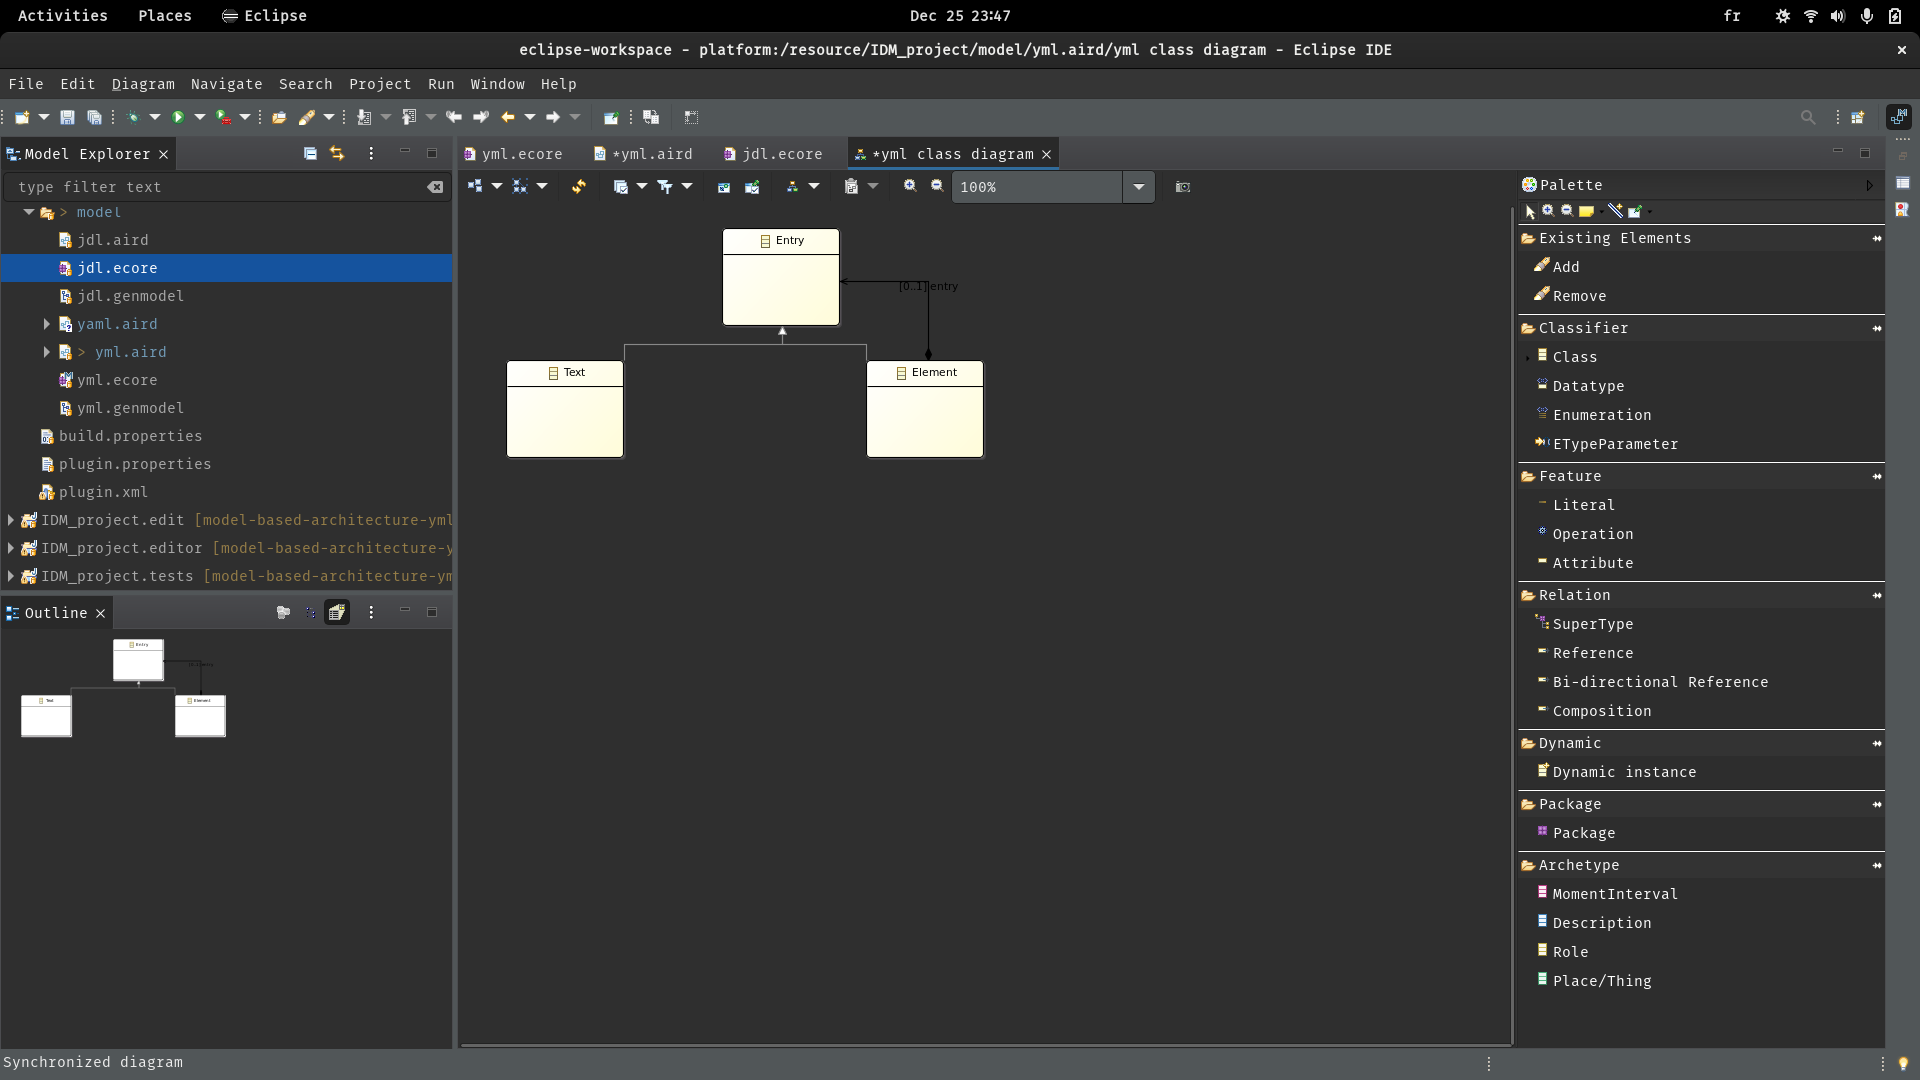
\includegraphics[width=16cm]{eclipse_yaml.png}
      }
      \caption{}
  \end{center}
\end{figure}